%!TEX program = xelatex
\documentclass[xcolor={table}]{beamer}

\usepackage[brazil]{babel}	
\usepackage[utf8]{inputenc}
\usepackage[T1]{fontenc}
\usepackage[scaled]{helvet}
\usepackage{amsthm}
\usepackage{ragged2e}
\usepackage{subfig}
\usepackage[table]{xcolor}
\usepackage{multicol}
\usepackage{multirow}
\usepackage{fancyvrb}
\usepackage{verbatim}
\usepackage{hyperref}
\definecolor{gold}{rgb}{0.81,0.69,0}
\definecolor{silver}{rgb}{0.75,0.75,0.75}
\usetheme{Execushares}

\title{Laborator 4 - PIT}
\subtitle{}
\author{Coca Mihai \\
        Ioana Dragoș}

\setcounter{showSlideNumbers}{1}

\begin{document}
	\setcounter{showProgressBar}{0}
	\setcounter{showSlideNumbers}{0}

	\frame{\titlepage}

	\begin{frame}
		\frametitle{Tabelă de Conținut}
		\begin{enumerate}
            \item Concepte teoretice
			\item Configurare
			\item Exemplu practic
		\end{enumerate}
	\end{frame}

	\setcounter{framenumber}{0}
	\setcounter{showProgressBar}{1}
	\setcounter{showSlideNumbers}{1}
	\section{Concepte teoretice}
	\begin{frame}
	    \frametitle{PIT}
	    \begin{itemize}
	        \item \textbf{\textit{Periodic Interrupt Timer}}
	        \item Acest periferic este reprezentat printr-un tablou de \textit{timere} care pot configurate programatic pentru generarea de întreruperi mascabile la perioade de timp specifice.
	        \item \textbf{\textit{Timer}} - numărător digital a cărui valoare configurată prin intermediul regiștrilor se modifică decremental la fiecare semnal de ceas
	        \item \textbf{\textit{Semnal de ceas}}
	        \begin{itemize}
	            \item \textbf{\textit{Perioada semnalului de ceas}} - $\frac{1}{\text{Frecvență BUS CLOCK}}$ \\
	            \item \textbf{\textit{Frecvență BUS CLOCK}} \sim 10.485.760 Hz \\
	        \end{itemize}
	        \item \textbf{\textit{Resetare timer}} -  Valoare configurată în registrul asociat * perioada semnalului de ceas. \\
	        
	    \end{itemize}
	\end{frame}
		\begin{frame}
	    \frametitle{Capabilități}
	    \begin{itemize}
	        \item \textbf{\textit{Periodic Interrupt Timer}}
	        \item Măsurarea unei perioade de timp
	        \item Numărarea unor evenimente
	        \item Generarea unor evenimente la perioade fixe de timp
	        \item Generarea unor forme de undă
	    \end{itemize}
	\end{frame}
			\begin{frame}
	    \frametitle{Mod de funcționare}
        \begin{figure}
            \centering
            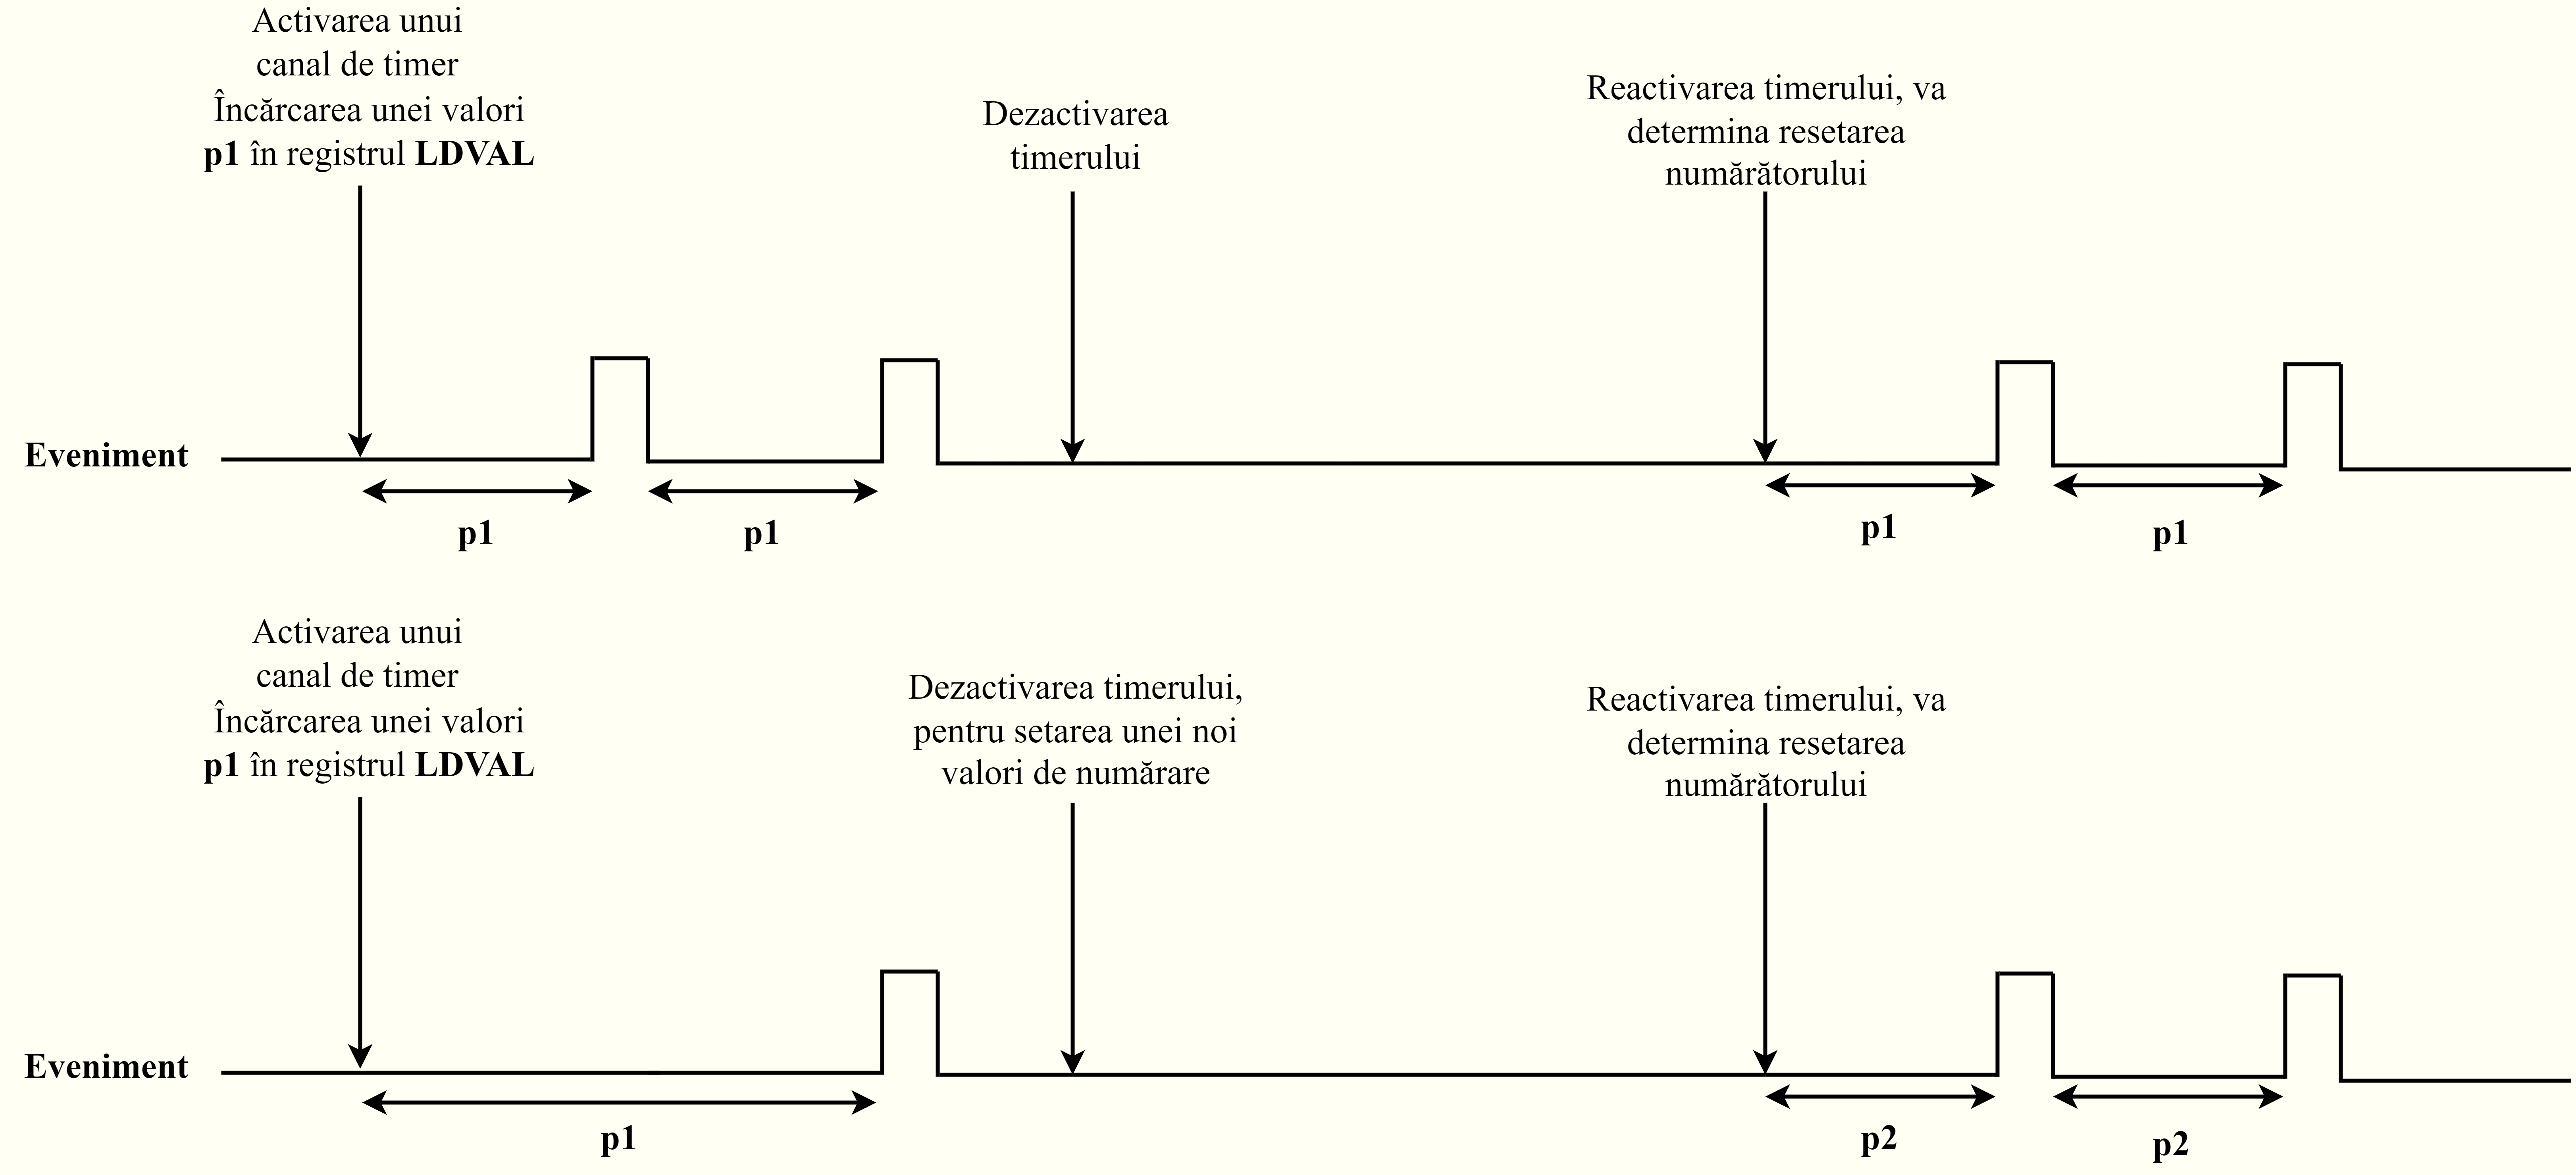
\includegraphics[width=11.5cm]{images/PIT.drawio (1).png}
            \caption{Generarea semnalelor prin intermediul perifericului PIT}
            \label{fig:my_label}
        \end{figure}
	\end{frame}
		\begin{frame}
	    \frametitle{Noțiuni introductive}
	    \begin{itemize}
	        \item \textbf{\textit{PIT FRDM-KL25Z}}
	        \begin{itemize}
	            \item Existența a două canale folosite pentru timere \\
	            (\textbf{\textit{Channel 0} și \textbf{\textit{Channel 1}}})
	            \item Fiecare timer are asociată o valoare de numărare independentă.
	            \item Accesul la un canal se face cu ajutorul sintaxei \textbf{\textit{PIT->CHANNEL[x]}}
	        \end{itemize}
	        \item Perifericul PIT nu interfațează cu pini externi.
	        
	    \end{itemize}
	\end{frame}
	\section{Configurare}
	\begin{frame}
	    \frametitle{\href{https://github.com/undacmic/MCULabs/blob/main/Resurse/FRDM-KL25Z_ReferenceManual.pdf}{Setarea regiștrilor}}
	    \begin{itemize}
	        \item Atunci când dorim să utilizăm un timer, pornirea acestuia, setarea și citirea valorii numărătorului se pot face într-o manieră programatică. 
	        \item Regiștrii care pun la dispoziție aceste setări:
	        \begin{itemize}
	            \item \textbf{\textit{PIT\_MCR}} - Module Control Register
	            \item \textbf{\textit{PIT\_LDVALx}} - Timer Load Value Register 
	            \item \textbf{\textit{PIT\_CVALx}} - Current Timer Value Register
	            \item \textbf{\textit{PIT\_TCTRLx}} - Timer Control Register
	            \item \textbf{\textit{PIT\_TFLGx}} - Timer Flag Register
	        \end{itemize}
	    \end{itemize}
	\end{frame}
		\begin{frame}
	    \frametitle{\href{https://github.com/undacmic/MCULabs/blob/main/Resurse/FRDM-KL25Z_ReferenceManual.pdf}{Setarea regiștrilor}}
	    \begin{itemize}
	        \item Activarea semnalului de ceas pentru a putea configura modulele folosite
	        \begin{itemize}
	            \item \textbf{\textit{SIM\_SCGC6}} - activarea modulului periferic \textbf{PIT}
	        \end{itemize}
	        \item \textbf{\textit{PIT\_MCR}} - utilizarea semnalului de ceas pentru timerele puse la dispoziție de PIT (\textbf{\textit{MDIS}}) și configurarea comportamentului timerelor la debug \textbf{(\textit{FRZ})}
	        \item \textbf{\textit{PIT\_LDVAL}} - configurarea valorii numărătorului se face pe baza formulei
	        \begin{align*}
	            \text{\textbf{Load Value = Nr. sec. * BUS CLOCK Freq. - 1}}
	        \end{align*}
	        \item \textbf{\textit{PIT\_TCTRL}} - permite activara/dezactivarea timerului(\textbf{\textit{TEN}}) de pe canalul asociat și a întreruperilor generate(\textbf{\textit{TIE}}).
	    \end{itemize}
	\end{frame}
			\begin{frame}
	    \frametitle{\href{https://github.com/undacmic/MCULabs/blob/main/Resurse/FRDM-KL25Z_ReferenceManual.pdf}{Setarea regiștrilor}}
	    \begin{itemize}
	        \item \textbf{\textit{PIT\_TFLG}} - verificarea câmpului \textbf{\textit{TIF}} pentru apariția unei întreruperi pe un anumit canal
	        \item \textbf{\textit{PIT\_LTMR}} - PIT Lifetime Timer Register permite crearea unui timer pe 64 de biți (separat pe doi regiștri) și prin utilizarea flag-ului \textbf{\textit{CHN}} din cadrul registrului \textbf{\textit{PIT\_TCTRL}} care permite înlănțuirea timerelor.
	        \begin{itemize}
	            \item \textbf{\textit{PIT\_LTMR64H}} - HIGH, corespunde cu \textbf{PIT->CHANNEL[1].CVAL}
	            \item \textbf{\textit{PIT\_LTMR64L}} - LOW, corespunde cu \textbf{PIT->CHANNEL[0].CVAL}
	            \item Pentru a fi decrementat canalul \textbf{\textit{n}} este nevoie de resetarea numărătorului de pe canalul \textbf{\textit{n-1}}.
	        \end{itemize}
	    \end{itemize}
	\end{frame}
	\section{Exemplu practic}
	\begin{frame}
	    \frametitle{Experiment}
	    \begin{itemize}
	        \item Dorim activarea ambelor canale PIT, pentru a folosi 2 numărătoare în paralel, fiecare cu o valoare diferită.
	        \item \textbf{\textit{Obiectiv: }} La interval de o secundă, să fie actualizat un cronometru afișat prin intermediul perifericului \textbf{\textit{UART}} la terminal. La interval de 10 secunde să aprindem un LED cu ajutorul perifericului \textbf{\textit{GPIO}}.
	        \item Încărcarea valorilor corespunzătoare în registrul \textbf{\textit{LDVAL}} pe baza formulei prezentate în laborator.
	        \item Avem nevoie de activarea înteruperilor pentru perifericul \textbf{\textit{PIT}} și suprascrierea handler-ului de întreruperi  \textbf{\textit{PIT\_IRQHandler}} pentru a avea o logică separată pentru cele două canale.
	        \item Realizarea conexiunii cu \textbf{GND}
	    \end{itemize}
	\end{frame}
		\begin{frame}
	    \frametitle{Rezultat}
	    \begin{figure}
	        \centering
	        \includegraphics[width=10cm]{images/circuit-pit.png}
	        \caption{Circuit electric final}
	        \label{fig:my_label}
	    \end{figure}
	\end{frame}
	\appendix


\end{document}